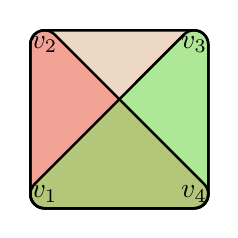
\begin{tikzpicture}[x=0.95cm,y=0.95cm]
  \fill[brown!80, fill opacity=0.38] (-0.190,0.000) arc[start angle=180.00, end angle=270.00, radius=0.19] -- (2.000,-0.190) arc[start angle=-90.00, end angle=0.00, radius=0.19] -- (2.190,2.000) arc[start angle=0.00, end angle=90.00, radius=0.19] -- (0.000,2.190) arc[start angle=90.00, end angle=180.00, radius=0.19] -- cycle;
  \fill[red!70, fill opacity=0.38] (-0.190,0.000) arc[start angle=180.00, end angle=270.00, radius=0.19] -- (2.000,-0.190) arc[start angle=-90.00, end angle=45.00, radius=0.19] -- (0.134,2.134) arc[start angle=45.00, end angle=180.00, radius=0.19] -- cycle;
  \fill[green!70, fill opacity=0.38] (-0.134,0.134) arc[start angle=135.00, end angle=270.00, radius=0.19] -- (2.000,-0.190) arc[start angle=-90.00, end angle=0.00, radius=0.19] -- (2.190,2.000) arc[start angle=0.00, end angle=135.00, radius=0.19] -- cycle;
  \draw[black, line width=0.9pt] (-0.190,0.000) arc[start angle=180.00, end angle=270.00, radius=0.19] -- (2.000,-0.190) arc[start angle=-90.00, end angle=0.00, radius=0.19] -- (2.190,2.000) arc[start angle=0.00, end angle=90.00, radius=0.19] -- (0.000,2.190) arc[start angle=90.00, end angle=180.00, radius=0.19] -- cycle;
  \draw[black, line width=0.9pt] (-0.190,0.000) arc[start angle=180.00, end angle=270.00, radius=0.19] -- (2.000,-0.190) arc[start angle=-90.00, end angle=45.00, radius=0.19] -- (0.134,2.134) arc[start angle=45.00, end angle=180.00, radius=0.19] -- cycle;
  \draw[black, line width=0.9pt] (-0.134,0.134) arc[start angle=135.00, end angle=270.00, radius=0.19] -- (2.000,-0.190) arc[start angle=-90.00, end angle=0.00, radius=0.19] -- (2.190,2.000) arc[start angle=0.00, end angle=135.00, radius=0.19] -- cycle;
  \node[inner sep=0pt] at (0.000,2.000) {$v_{2}$};
  \node[inner sep=0pt] at (2.000,2.000) {$v_{3}$};
  \node[inner sep=0pt] at (0.000,0.000) {$v_{1}$};
  \node[inner sep=0pt] at (2.000,0.000) {$v_{4}$};
\end{tikzpicture}
